
%	Documentação do Trabalho Prático 1 de AEDSIII
%	@Sandro Miccoli
%
%	* Você pode identificar erros de grafia através do seguinte comando linux:
%		aspell --encoding="utf-8" -c -t=tex --lang="pt_BR" tp1.tex
%

\documentclass[12pt]{article}
\usepackage{sbc-template}
\usepackage{graphicx}
\usepackage{latexsym}
\usepackage{subfigure}
\usepackage{times,amsmath,epsfig}
\usepackage{graphicx,url}
 \makeatletter
 \newif\if@restonecol
 \makeatother
 \let\algorithm\relax
 \let\endalgorithm\relax
\graphicspath{{./data/}}
\usepackage[lined,algonl,ruled]{algorithm2e}
\usepackage{multirow}
\usepackage[brazil]{babel}
\usepackage[utf8]{inputenc}
\usepackage{listings}

\usepackage{alltt}
\renewcommand{\ttdefault}{txtt}

\sloppy

\title{TRABALHO PRÁTICO 1: \\ Grafos}

\author{Sandro Miccoli - 2009052409 - smiccoli@dcc.ufmg.br}

\address{Departamento de Ciência da Computação -- Universidade Federal de Minas Gerais (UFMG)\\
\\
\today}


\begin{document}

\maketitle

\begin{resumo}
Esse relatório descreve como foi foi solucionado o problema proposto no Trabalho Prático 1, o qual será detalhado ao longo das próximas seções. Será descrito também a modelagem do problema e a solução proposta para tal. Finalmente será detalhado a análise de complexidade dos algoritmos, os testes utilizados para comprovar tais análises e uma breve conclusão do trabalho implementado.
\end{resumo}

\section{INTRODUÇÃO}

	A situação que deparamos neste trabalho é a seguinte: a distribuidora de produtos, Atlanticon, está precisando de uma consultoria para decidir em qual cidade deve instalar a nova filial para servir uma determinada região.

	A empresa possui conhecimento das distâncias entre quaisquer duas cidades da região que sejam conectadas por algum trilho. Além disso, o trem, precariamente, realiza a entrega de apenas um produto por viagem, tornando necessário retornar para a filial para carregar um novo produto.

	Existem 3 cenários distintos que a Atlanticon deseja saber qual a melhor opção de cidade para instalar a nova filial, e o objetivo do trabalho é solucionar esse problema.

	Descreveremos aqui os três cenários:

	\textbf{Cenário 1: } Escolher a cidade de modo a minimizar os custos de gasto em combustível. Considerando que cada cidade emite a mesma quantidade de pedidos em um mesmo intervalo de tempo.

	\textbf{Cenário 2: } Escolher a cidade para também minimizar os custos de gasto em combustível. Porém, neste cenário cada cidade possui um volume diferente de pedidos, isso deve ser considerado para a escolha final.

	\textbf{Cenário 3: } A Atlanticon deseja garantir que o produto seja entregue num prazo de $X$ horas. A escolha da cidade se dá pelo menor valor possível de $X$ que pudermos encontrar.

	O restante deste relatório é organizado da seguinte forma. A Seção~\ref{modelagem} descreve como foi feita a modelagem e manipulação dos grafos. A Seção \ref{solucao_proposta} descreve rapidamente qual foi a solução proposta além do método utilizado para calcular as distâncias mínimas entre as cidades. A Seção~\ref{implementacao} trata de detalhes específicos da implementação do trabalho: quais os arquivos utilizados; como é feita a compilação e execução; além de detalhar o formato dos arquivos de entrada e saída. A Seção~\ref{avaliacao_experimental} contém a avaliação experimental, quantificando o tempo de execução de cada operação com grafos de diversos tamanhos e formatos. A Seção~\ref{conclusao} conclui o trabalho.


\section{MODELAGEM}
\label{modelagem}

	Inicialmente, para trabalhar com grafos, foi criada uma estrutura que contém a informação de quantos vértices o grafo possui, nesse caso, cidades, e qual o volume de pedidos de cada cidade:

    \begin{lstlisting}[language=c]
    typedef struct grafo {
        Matriz matrizAdj;
        int N; // Quantidade de cidades no grafo
        int *Vol; // Volume de pedidos de cada cidade
    } Grafo;

    typedef struct Matriz{
        int col, lin;
        int ** matriz;
    } Matriz;

    \end{lstlisting}

    Já que o grafo que nos é passado como entrada é uma matriz de adjacências, e como já havíamos implementado uma estrutura de matriz no Trabalho Prático 0, reutilizamos o código neste trabalho.

	A complexidade de espaço dessa estrutura pode ser considerada como $O(n)$, sendo $n$ o tamanho bidimensional da matriz, ou seja, o produto entre a quantidade de linhas e colunas que ela possui.

	Como foi detalhado na especificação, a matriz foi modelada para ser alocada e desalocada dinâmicamente, através dos comandos \textit{malloc} e \textit{free}. Para confirmar que este processo de alocação dinâmica de memória estava ocorrendo como esperado, foi utilizado o comando \textit{valgrind} para verificar qualquer tipo de vazamento de memória.

\section{SOLUÇÃO PROPOSTA}
\label{solucao_proposta}

	O problema que deparamos é minimizar o custo de combustível dos trens da empresa Atlanticon. Como já modelamos nosso problema como um grafo, nada melhor que um algoritmo específico que nos traga a solução. A seguir uma definição de \cite{sedgewick} para o problema de caminho mínimo:

	\begin{quote}
	Dado um digrafo com custos não negativos nos arcos e um vértice \textit{s}, encontrar uma arborescência de caminhos mínimos com raiz \textit{s} no digrafo.
	\end{quote}

	O algoritmo que utilizaremos foi inventado por Edsger Dijkstra [a pronúncia é algo entre "Dêcstra"\ e "Dêicstra"] e publicado em 1959. O algoritmo pode ser usado, em particular, para encontrar um caminho de custo mínimo de um dado vértice a outro \cite{sedgewick}.

	A solução proposta aqui foi realizar o algoritmo de Dijkstra para cada vértice do grafo, então descobrir o menor caminho dentre todos os possíveis para resolver nosso problema de distribuição de produtos pelas linhas de trem.

	Para o \textbf{Cenário 1} utilizamos apenas as distâncias entre as cidades como peso nas arestas para calcular o caminho mínimo entre os vértices.

	Já no \textbf{Cenário 2}, para cada cidade, calculamos o produto entre a distância das cidades com o volume de pedidos de cada uma. O menor produto resulta na nossa melhor escolha.

	No \textbf{Cenário 3}, temos que minimizar o valor de $X$, para isso inicialmente calculamos a maior distância percorrida para cada cidade. Assim garantimos a quantidade de horas mínima para o pedido chegar. Dentre essas maiores distâncias, escolhemos a menor delas, minimizando o valor de $X$.

	Além desses cenários, tempos que retornar qual o prejuízo percentual acarretado quando a cidade é escolhida, de modo a garantir o menor tempo de entrega máximo. Para isso calculamos a razão entre os custos do \textbf{Cenário 1} e \textbf{Cenário 3}. Isso nos retorna qual a porcentagem de aumento de combustível caso a Atlanticon escolher a cidade do \textbf{Cenário 3} para implantar a filial.

\subsection{Principais funções implementadas}

\subsubsection{Dijkstra}

\begin{itemize}
 \item \begin{large}\textit{void dijkstra (Grafo G, int v,  int *dis)}\end{large}\\
 \subitem \textbf{Descrição:} Soluciona o problema do caminho mais curto para o vértice $v$ e armazena o resultado no vetor de distâncias dis.
 \subitem \textbf{Parâmetros:} Estrutura de grafo $G$, vértice $v$ e vetor de distâncias $dis$.
 \subitem \textbf{Complexidade:} $O(n^2)$, onde $n$ são os vértices do grafo.
\end{itemize}

\vspace{0.2 true cm}

\begin{itemize}
 \item \begin{large}\textit{void dijkstra\_all (Grafo G)}\end{large}\\
 \subitem \textbf{Descrição:} Soluciona o problema do caminho mais curto para todos os vértices do grafo e atualiza a matriz de adjacência contida no grafo transformando-a em uma matriz de distâncias mínimas.
 \subitem \textbf{Parâmetros:} Estrutura de grafo $G$.
 \subitem \textbf{Complexidade:} $O(n^3)$, onde $n$ são os vértices do grafo.
\end{itemize}


\subsubsection{Consultoria}

\begin{itemize}
 \item \begin{large}\textit{int cenarioUm(Grafo G)}\end{large}\\
 \subitem \textbf{Descrição:} Pesquisa no grafo $G$, que agora contém uma matriz de distâncias mínimas, para descobrir qual cidade possui o menor caminho a ser percorrido pelo grafo. Retorna o índice da melhor cidade.
 \subitem \textbf{Parâmetros:} Estrutura de grafo $G$.
 \subitem \textbf{Complexidade:} $O(n^2)$, onde $n$ são os vértices do grafo.
\end{itemize}

\vspace{0.2 true cm}

\begin{itemize}
 \item \begin{large}\textit{int cenarioDois(Grafo G)}\end{large}\\
 \subitem \textbf{Descrição:} Vasculha o grafo $G$, que agora contém uma matriz de distâncias mínimas, para descobrir qual cidade possui o menor caminho a ser percorrido pelo grafo. Porém, agora considerando o volume médio de pedidos de cada cidade. Retorna o índice da melhor cidade.
 \subitem \textbf{Parâmetros:} Estrutura de grafo $G$.
 \subitem \textbf{Complexidade:} $O(n^2)$, onde $n$ são os vértices do grafo.
\end{itemize}

\vspace{0.2 true cm}

\begin{itemize}
 \item \begin{large}\textit{int cenarioTres(Grafo G)}\end{large}\\
 \subitem \textbf{Descrição:} Caminha pelo grafo $G$, que agora contém uma matriz de distâncias mínimas, para descobrir qual o menor caminho dentre os maiores caminhos percorridos de cada cidade. Retorna o índice da melhor cidade.
 \subitem \textbf{Parâmetros:} Estrutura de grafo $G$.
 \subitem \textbf{Complexidade:} $O(n^2)$, onde $n$ são os vértices do grafo.
\end{itemize}

\vspace{0.2 true cm}

\begin{itemize}
 \item \begin{large}\textit{float prejuizoCen3(Grafo G, int cen1, int cen3)}\end{large}\\
 \subitem \textbf{Descrição:} Calcula o custo do cenário 1 para a cidade de índice $cen1$ e do cenário 3 para a cidade de índice $cen3$. Depois é calculado a razão entre esses custos e esse é o prejuízo de se escolher o cenário 3 em vez do 1. O valor retornado é um $float$ contendo o prejuízo em porcentagem.
 \subitem \textbf{Parâmetros:} Estrutura de grafo $G$, índice da cidade do cenário 1 $cen1$, índice da cidade do cenário 3 $cen3$.
 \subitem \textbf{Complexidade:} $O(n)$, onde $n$ são os vértices do grafo.
\end{itemize}


\section{IMPLEMENTAÇÃO}
\label{implementacao}

\subsection{Código}

\subsubsection{Arquivos .c}

\begin{itemize}
\item \textbf{tp1.c} Arquivo principal do programa, lê todas as instâncias de problemas do arquivo de entrada, realiza os cálculos dos cenários e insere cada resultado no arquivo de saída.
\item \textbf{matriz.c} Contém todas as funções de manipulação, leitura e escrita de matrizes.
\item \textbf{grafos\_matriz.c} Contém todas as funções de manipulação, leitura e escrita de grafos. Utiliza o TAD de matriz como implementação da matriz de adjacências.
\item \textbf{dijkstra.c} Contém a implementação do algoritmo de Dijkstra, tanto para um vértice quanto para todos os vértices do grafo.
\item \textbf{consultoria.c} Contém a implementação de todos os cenários que a Atlanticon estabeleceu.
\end{itemize}

\subsubsection{Arquivos .h}

\begin{itemize}
\item \textbf{matriz.h} Além de definir a estrutura de matriz, contém o cabeçalho todas as funções de manipulação, leitura e escrita de matrizes.
\item \textbf{grafos\_matriz.h} Além de definir a estrutura de grafos, contém todas as funções de manipulação, leitura e escrita de grafos. Utiliza o TAD de matriz como implementação da matriz de adjacências.
\item \textbf{dijkstra.h} Contém o cabeçalho do algoritmo de Dijkstra, tanto para um vértice quanto para todos os vértices do grafo.
\item \textbf{consultoria.h} Contém o cabeçalho de todos os cenários que a Atlanticon estabeleceu.
\end{itemize}

\subsection{Compilação}

O programa deve ser compilado através do compilador GCC através de um makefile ou do seguinte comando:

\begin{footnotesize}
\begin{verbatim}
gcc -Wall -Lsrc src/tp1.c src/arquivos.c src/grafos_matriz.c
                src/matriz.c src/dijkstra.c src/consultoria.c -o tp1 \end{verbatim}
\end{footnotesize}

Ou através do comando $make$.

\subsection{Execução}

A execução do programa tem como parâmetros:
\begin{itemize}
\item Um arquivo de entrada contendo várias instâncias de grafos e seus respectivos volumes de pedidos pra cada cidade.
\item Um arquivo de saída que irá receber o resultado dos cálculos de cada cenário e o percentual de prejuízo, já explicado na Seção~\ref{solucao_proposta}.
\end{itemize}

O comando para a execução do programa é da forma:

\begin{footnotesize}
\begin{verbatim} ./tp1 <arquivo_de_entrada> <arquivo_de_saída>\end{verbatim}
\end{footnotesize}

\subsubsection{Formato da entrada}

A primeira linha do arquivo de entrada contém o valor \textit{k} de instâncias que o arquivo contém. A próxima linha contém a quantidade \textit{n} de cidades que o grafo contém. As próximas \textit{m} linhas contém a matriz de adjacência referente à esse grafo. Por último, a última linha contém \textit{n} inteiros que são referentes ao volume médio de pedidos de cada cidade da região.

A Figura~\ref{grafo} contém um grafo com 7 cidades, esparso. Geramos um arquivo que contém a matriz de adjacência dele e o volume de pedidos de cada cidade. Esse arquivo de entrada tem a seguinte configuração:

\begin{figure}[h!]
	\centering
	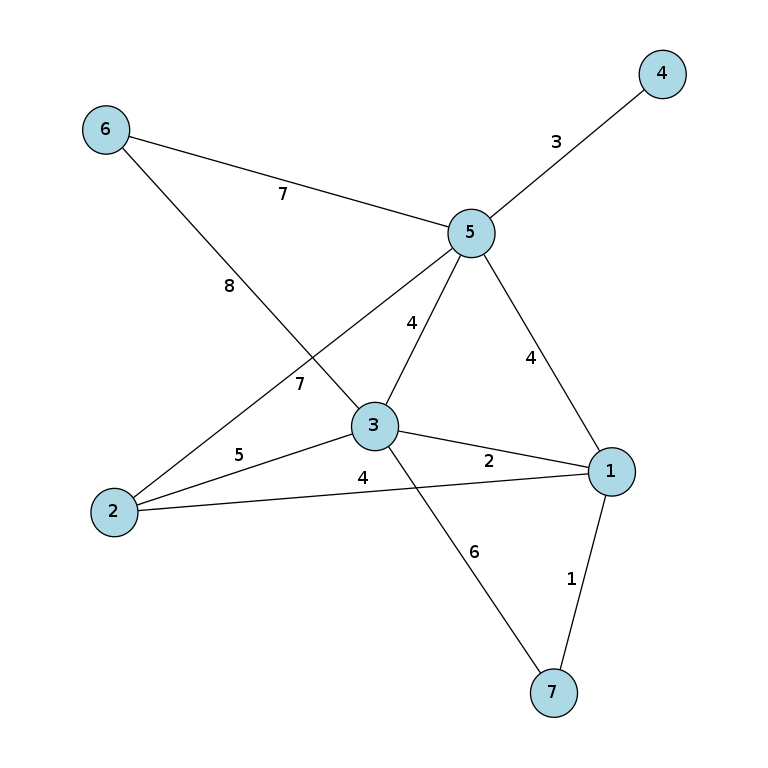
\includegraphics[width=.8\textwidth]{graph_teste.png}
	\caption{Grafo esparso com 7 cidades}
	\label{grafo}
\end{figure}


\begin{verbatim}
1
7
0 4 2 0 4 0 1
4 0 5 0 7 0 0
2 5 0 0 4 8 6
0 0 0 0 3 0 0
4 7 4 3 0 7 0
0 0 8 0 7 0 0
1 0 6 0 0 0 0
217 730 272 684 339 890 356
\end{verbatim}

\subsubsection{Formato da saída}

O arquivo de saída contém 3 inteiros e um valor de ponto flutuante. Cada inteiro é um identificador da cidade na qual a filial deve ser instalado considerando cada um dos cenários descritos na Seção~\ref{solucao_proposta}. O último valor consiste no aumento percentual ao se escolher a cidade de modo a minimizar o tempo máximo de entrega ao invés de minimizar o gasto total de combustível.

Considerando o grafo da Figura~\ref{grafo}, o resultado obtido após a execução do programa é escrito no arquivo de saída, que tem a seguinte configuração:

\begin{verbatim}
1 5 5 7.14
\end{verbatim}


\section{AVALIAÇÃO EXPERIMENTAL}
\label{avaliacao_experimental}

Para testar o algoritimo realizamos quatro testes, separados em dois grupos. O primeiro grupo de testes se refere à grafos esparsos e o segundo a grafos densos.

Para cada grupo de testes fizemos um teste que varia a quantidade instâncias, com grafos de tamanho fixo (25 vértices), e outro teste com apenas uma instância e grafos de tamanhos crescentes.

\subsection{Máquina utilizada}
\label{maquina}

Segue especificação da máquina utilizada para os testes:
\begin{verbatim}
model name:     Intel(R) Core(TM) i3 CPU       M 330  @ 2.13GHz
cpu MHz:        933.000
cache size:     3072 KB
MemTotal:       3980124 kB
\end{verbatim}

\subsection{Grafos Esparsos - Variando quantidade de instâncias}
\label{esparsos_inst}

	Na Figura \ref{esp_inst_var}, é possível ver o tempo de execução para o primeiro teste. Aqui fixamos o tamanho do grafo para 25 vértices e variamos o número de instâncias, de 1 até 500. O maior tempo foi de $34$ segundos, para 500 instâncias.

\begin{figure}[h!]
	\centering
	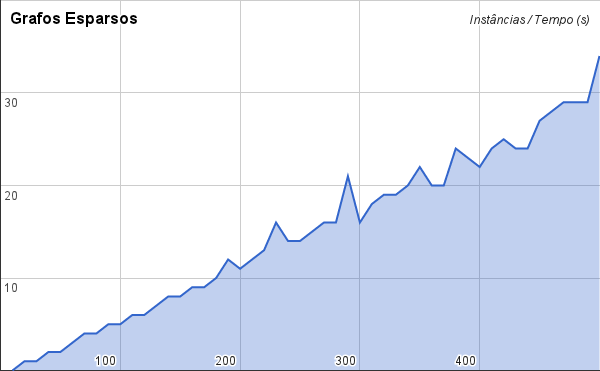
\includegraphics[width=0.60\textwidth]{graph_esparso_instvar.png}
	\caption{Grafos esparsos com instâncias variando até 500}
	\label{esp_inst_var}
\end{figure}

\subsection{Grafos Esparsos - Variando tamanho dos grafos}
\label{esparsos_graf}

	Na Figura \ref{esp_graf_var}, é possível ver o tempo de execução para o segundo teste. Aqui fixamos quantidade de instâncias para apenas uma, e variamos a quantidade de vértices do grafo, que foi de 1 até 500. O maior tempo de execução foi de $246$ segundos, para 500 vértices.

\begin{figure}[h!]
	\centering
	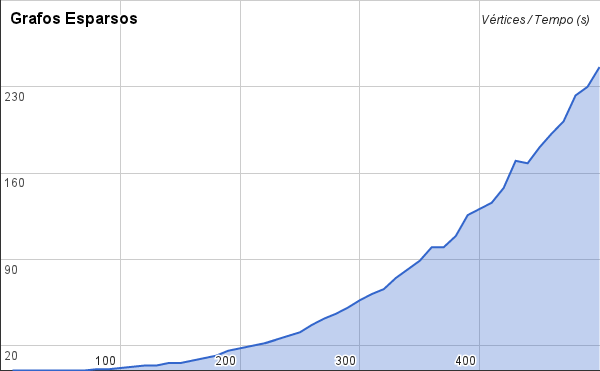
\includegraphics[width=0.60\textwidth]{graph_esparso_grafvar.png}
	\caption{Grafos esparsos com grafos variando até 500 vértices}
	\label{esp_graf_var}
\end{figure}

\subsection{Grafos Densos - Variando quantidade de instâncias}
\label{densos_inst}

	Na Figura \ref{den_inst_var}, é possível ver o tempo de execução para o terceiro teste. Aqui fixamos o tamanho do grafo para 25 vértices e variamos o número de instâncias, de 1 até 500. O maior tempo foi de $30$ segundos, para 500 instâncias.

\begin{figure}[h!]
	\centering
	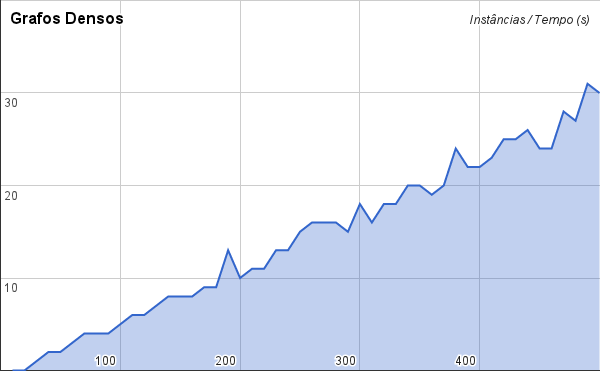
\includegraphics[width=0.60\textwidth]{graph_denso_instvar.png}
	\caption{Grafos densos com instâncias variando até 500}
	\label{den_inst_var}
\end{figure}

\subsection{Grafos Densos - Variando tamanho dos grafos}
\label{densos_graf}

	Na Figura \ref{den_graf_var}, é possível ver o tempo de execução para o quarto e último teste. Aqui fixamos quantidade de instâncias para apenas uma, e variamos a quantidade de vértices do grafo, que foi de 1 até 500. O maior tempo de execução foi de $224$ segundos, para 500 vértices.

\begin{figure}[h!]
	\centering
	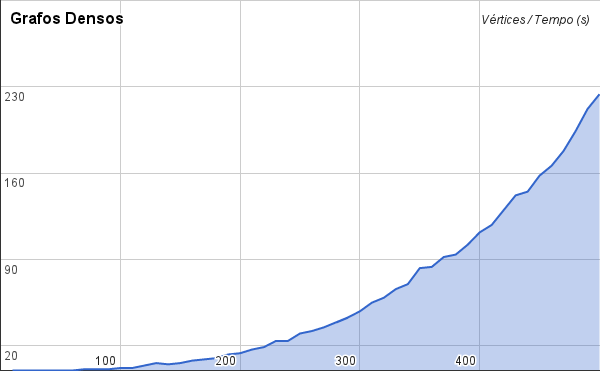
\includegraphics[width=0.60\textwidth]{graph_denso_grafvar.png}
	\caption{Grafos densos com grafos variando até 500 vértices}
	\label{den_graf_var}
\end{figure}

\subsection{Resultado}

	O resultado geral dos testes ocorreu como esperado. Os testes em que foi variada apenas as instâncias (\ref{esparsos_inst} e \ref{densos_inst}) cresceu de forma esperada, em um comportamento quase que constante.

    Já os testes em que variamos os tamanhos dos grafos (\ref{esparsos_graf} e \ref{densos_graf}) já deu pra visualizar melhor a complexidade do algoritmo de Dijkstra. Pelos gráficos é perceptível o crescimento exponencial de cada teste.

    Outra conclusão interessante é perceber que o Dijkstra que foi implementado neste trabalho funciona melhor para grafos densos do que para grafos mais esparsos. Veja a Figura \ref{graf_var} para uma melhor comparação entre os testes \ref{esparsos_graf} e \ref{densos_graf}.

    \begin{figure}[h!]
        \centering
        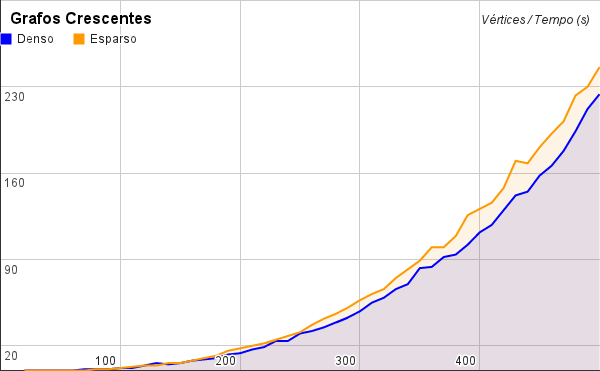
\includegraphics[width=0.80\textwidth]{graph_grafvar.png}
        \caption{Grafos densos e esparsos com grafos variando até 500 vértices}
        \label{graf_var}
    \end{figure}

\section{CONCLUSÃO}
\label{conclusao}

	O problema de calcular o produto de Kronecker das matriz foi solucionado sem muitas complicações. As matrizes foram alocadas dinâmicamente com sucesso, de acordo com o \textit{Valgrind}. Além disso, um padrão de código bem modularizado foi seguido, para que os módulos possam ser reutilizados futuramente.

	O código também já foi construído de uma maneira em que, caso futuramente seja necessário paralelizá-lo, poucas mudanças no código precisarão ser feitas para tal.

	Os testes foram bem sucedidos pois o tempo de processamento do algoritmo em diversas situações ocorreu como esperado.

	As primitivas básicas da linguagem C, como alocação dinâmica de memória e manipulação de arquivos, foram bem exploradas no trabalho prático. Além disso, procurei construir uma documentação bem detalhada sobre toda a estrutura e funcionamento do programa implementado.

\bibliographystyle{sbc}
\bibliography{tp1}

\end{document}
